\section{Theoretical Model}
  \label{sec:twophoton_theory}

    We wish to investigate population of the $5\rm{D}$ doublet states which lie
    close to two-photon resonance as the high-intensity laser is scanned across
    the \textsc{d2} lines, and subsequent population of the $6\rm{P}$ states via
    decay. We will need to consider light coupling the
    $5^2\rm{S}_{\nicefrac{1}{2}}$ ground state to the
    $5^2\rm{P}_{\nicefrac{1}{2}}$ and $5^2\rm{S}_{\nicefrac{3}{2}}$ states, and
    then coupling those intermediate states up to the
    $5^2\rm{D}_{\nicefrac{3}{2}}$ and $5^2\rm{D}_{\nicefrac{5}{2}}$ via 
    two-photon excitation. The model will then incorporate the
    $6^2\rm{P}_{\nicefrac{1}{2}}$ and $6^2\rm{P}_{\nicefrac{3}{2}}$ levels after
    decay from the $5\rm{D}$ states. Decay from the $6\rm{P}$ doublet back down
    to the $5^2\rm{S}_{\nicefrac{1}{2}}$ ground state is the channel responsible
    for the blue fluorescence.

    \begin{figure}[]
    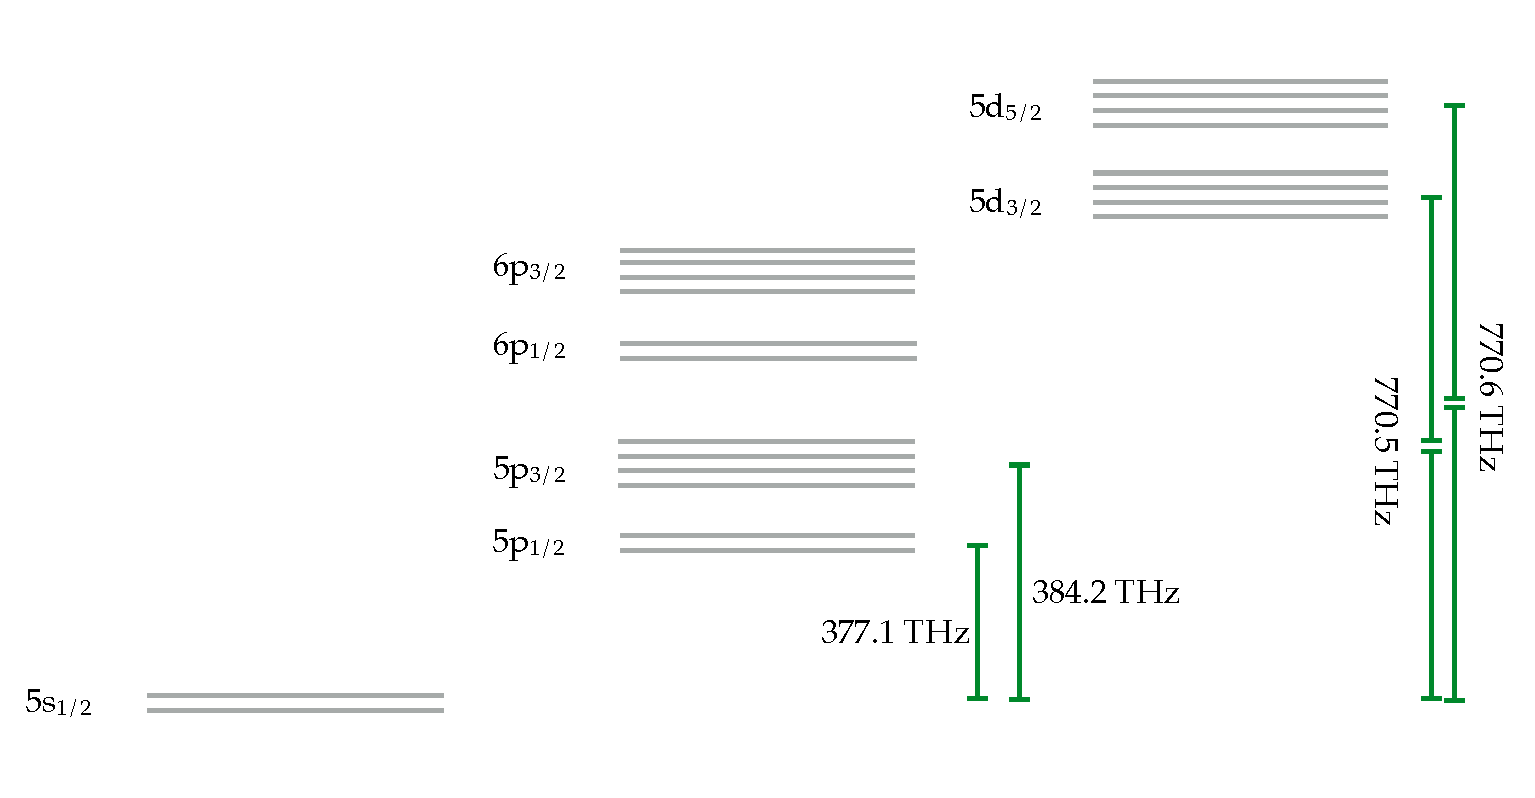
\includegraphics[width=\linewidth]
        {figs/05_twophoton/twophoton_level_scheme.pdf}
    \caption{
    Hyperfine structure of selected manifolds of rubidium 87. Frequencies of the
    $5^2\rm{S}_{\nicefrac{1}{2}} \rightarrow 5^2\rm{P}_{\nicefrac{1}{2}}$
    (\textsc{d1}) and $5^2\rm{S}_{\nicefrac{1}{2}} \rightarrow
    5^2\rm{P}_{\nicefrac{3}{2}}$ (\textsc{d2}) transitions are shown, along with
    the $5^2\rm{S}_{\nicefrac{3}{2}} \rightarrow 5^2\rm{D}_{\nicefrac{3}{2}}$
    and  $5^2\rm{S}_{\nicefrac{3}{2}} \rightarrow 5^2\rm{D}_{\nicefrac{5}{2}}$
    transitions, close to two-photon resonance on \textsc{d2}.
    } 
    \label{fig:two_photon_level_scheme} 
    \end{figure}

    The fine structure manifolds included in the model and their hyperfine
    levels are illustrated in figure \ref{fig:two_photon_level_scheme}.
    Experimentally measured values for the transition frequencies to these
    manifolds from the ground state are listed in table
    \ref{tab:exp_fine_energies}.

    In order to investigate the cause of the fluorescence at the scanning
    resolution of the experiment, as well as to include the effect of pumping
    mechanisms, our state basis must include the hyperfine structure and
    magnetic substructure of these fine structure manifolds, consisting of $2F +
    1$ degenerate sublevels $m_F = -F, -F + 1, \dots, F -1, F$ within each
    hyperfine level.

    \begin{table}
      \centering
      \begin{tabular}{ l r r r }
        \hline
        Manifold ($J'$) & Energy & $A_{\rm{hf}}$ for $^{87}$Rb 
          & $A_{\rm{hf}}$ for $^{85}$Rb \\
        \hline      
        $5^2\rm{S}_{\nicefrac{1}{2}}$ & $0.0$ & $3,417.34$ & $1,011.91$ \\
        \noalign{\medskip}
        $5^2\rm{P}_{\nicefrac{1}{2}}$ & $377.1074$ & $406.20$ & $120.53$ \\
        $5^2\rm{P}_{\nicefrac{3}{2}}$ & $384.2304$ & $84.85$ & $25.00$ \\
        \noalign{\medskip}
        $6^2\rm{P}_{\nicefrac{1}{2}}$ & $710.9602$ & $132.56$ & $39.12$ \\
        $6^2\rm{P}_{\nicefrac{3}{2}}$ & $713.2839$ & $27.70 $ & $8.16$ \\
        \noalign{\medskip}
        $5^2\rm{D}_{\nicefrac{3}{2}}$ & $770.4827$ & $14.43$ & $4.18$ \\
        $5^2\rm{D}_{\nicefrac{5}{2}}$ & $770.5715$ & $−7.44$ & $-2.19$ \\
        % \noalign{\medskip}
        \hline  
      \end{tabular}
      \caption{
      Experimental values of transition frequencies (in \unit{$2\pi$ THz}) for
      selected energy levels of rubidium, along with hyperfine constants
      $A_{\rm{hf}}$ (in \unit{$2\pi$ MHz}) for the $85$ and $87$ isotopes. See
      equation (\ref{eqn:twophoton_energy_shifts}) for the definition of
      $A_{\rm{hf}}$. Values are from \textsc{nist} data, recorded in Sansonetti,
      2006. \cite{Sansonetti2006}. $A_{\rm{hf}}$ values are from Arimondo, 1977
      and Banarjee, 2007.\cite{Arimondo1977, Banerjee2007}
      }
      \label{tab:exp_fine_energies}
    \end{table}

    The classical description of the high-intensity field is as we saw for a
    two-level atomic model in chapter \ref{chp:propagation}, consisting of a monochromatic electric field
    \begin{equation}
      \mathbf{E}(z,t) = \tfrac{1}{2} \mathbf{\hat{x}}  \left[ \mathcal{E}(z,t) 
          \ee^{\ii(k z - \omega t)} + \mathcal{E}^*(z,t) 
          \ee^{-\ii(k z - \omega t)} \right]
      \label{eqn:high_int_E_field}
    \end{equation}
    where once again $\mathbf{\hat{x}}$ is the polarisation vector of the fields
    and the envelope $\mathcal{E}(z,t)$ is a complex function.

    As in the case of the two- and three-level systems described in chapters
    \ref{chp:propagation} and \ref{chp:nonlinear}, in order to solve for the
    time evolution of the atomic system during interaction with the field of
    equation (\ref{eqn:high_int_E_field}), we must define the dipole operator by
    determining the transition dipole matrix elements coupling states of the
    atomic basis. First we will define the atomic basis and the bare Hamiltonian
    with the inclusion of atomic angular momentum structure.

  \subsection{Angular Momentum Structure}  

    The bare atomic Hamiltonian for the hydrogenic description of a rubidium
    atom represents the state of the valence electron prior to interaction with
    the optical field.

    The bare atomic Hamiltonian for the hydrogenic description of a rubidium
    atom represents the state of the valence electron prior to interaction with
    the optical field.

    Our basis consists of the set of all hyperfine sublevels contained in the
    fine structure manifolds in the model, indexed by quantum numbers $n$ and
    $J$. The bare atomic Hamiltonian in the hyperfine basis is then given by the
    sum of projection operators for those hyperfine sublevels, resulting in a
    diagonal operator
    \begin{align}
      \mathcal{H}_0 = &\hbar \sum_{F m_F} \delta \omega_F 
                        \Ket{F m_F} \Bra{F m_F} + \nonumber \\
      &\hbar \sum_{n' J'} \sum_{F' m_F'} (\omega_{n' J'} + 
        \delta \omega_{n' J', F'}) \Ket{F' m'_F} \Bra{F' m'_F}
    \end{align}
    where $F$ and $m_F$ index the ground state hyperfine sublevels and $\delta
    \omega_F$ values represent the energy shifts of the hyperfine levels
    relative to  the centre of gravity of the ground state manifold. Similarly,
    $F'$ and $m_F'$ index the excited state hyperfine sublevels and $\delta
    \omega_{n' J', F'}$ represent the energy shifts relative to the the centre
    of gravity of those excited state manifolds given by $\omega_{n' J'}$, the
    transition frequency from the ground state manifold to each state, listed in
    table \ref{tab:exp_fine_energies}.

    The energy shifts $\delta \omega_{n' J', F'}$ express coupling between the
    total electronic angular momentum $\bf{J}$ and the nuclear angular momentum
    $\bf{I}$, and to first order can be expressed via
    \begin{equation}
      \delta \omega_{n' J', F'} = 
        \frac{A_{\rm{hf}}}{\hbar^2} \left( \bf{I} \cdot \bf{J} \right)
        \label{eqn:twophoton_energy_shifts}
    \end{equation}
    where the values $A_{\rm{hf}}$ are (magnetic dipole) hyperfine constants,
    also listed in table \ref{tab:exp_fine_energies}. We shall neglect 
    higher-order corrections, including electric quadrupole coupling, in this 
    model as the energy shifts are relatively small.

    \begin{figure}[]
    \centering
    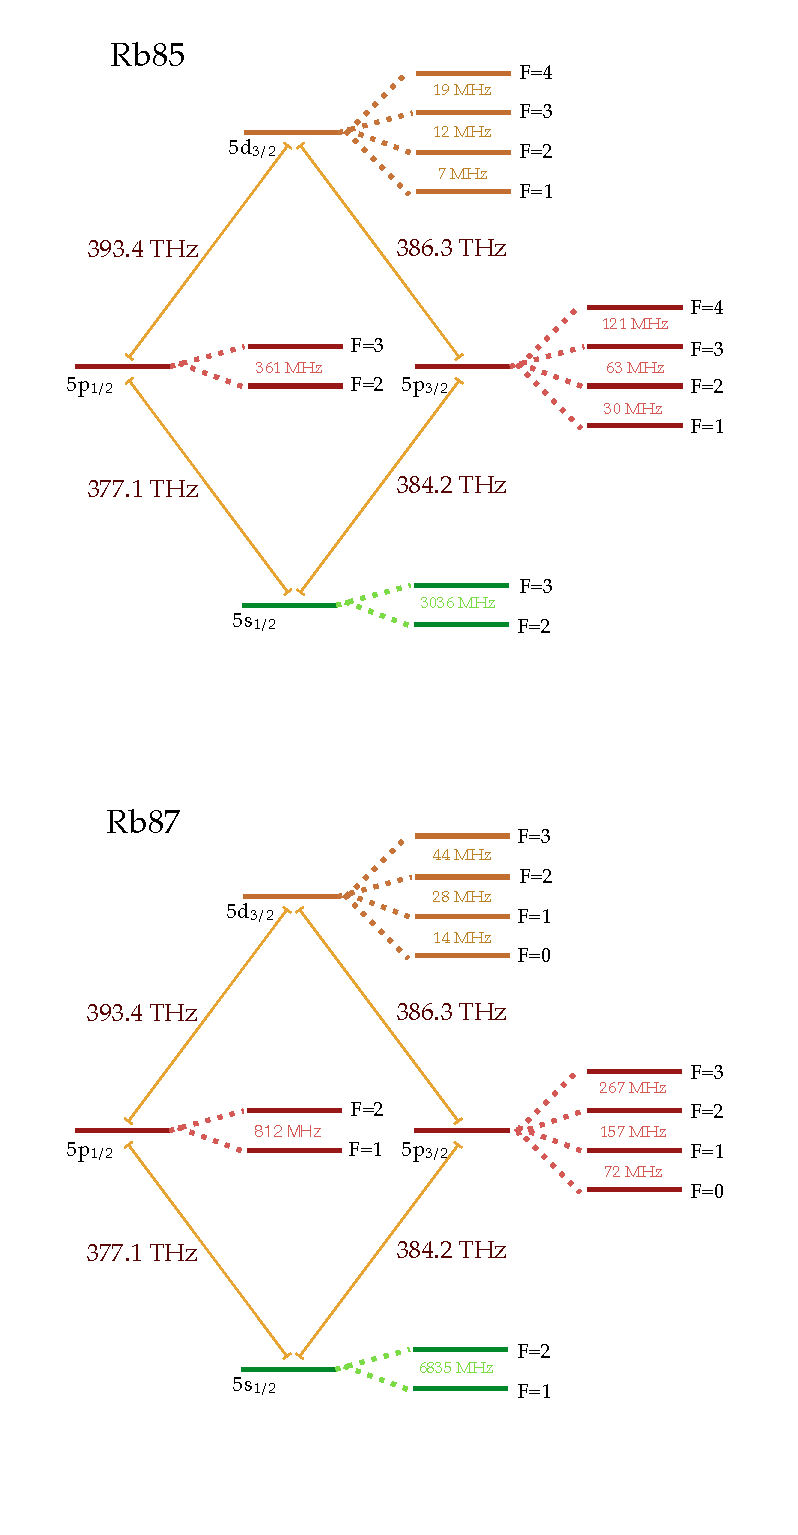
\includegraphics[width=0.7\linewidth]
        {figs/05_twophoton/5spd_energy_levels_vert.pdf}
    \caption{
    Hyperfine splittings of the $5^2\rm{S}_{\nicefrac{1}{2}}$,
    $5^2\rm{P}_{\nicefrac{1}{2}}$ $5^2\rm{P}_{\nicefrac{3}{2}}$ and
    $5^2\rm{D}_{\nicefrac{3}{2}}$ levels in rubidium, for both isotopes, $85$
    and $87$, showing the two-photon coupling and transition frequencies. Each
    hyperfine level consists of $2F + 1$ degenerate sublevels. These splittings
    are determined from the experimental values given and referenced in table
    \ref{tab:exp_fine_energies}.
    }
    \label{fig:5spd_energy_levels}
    \end{figure}

    % [TODO: Make bigger: two rows instead of two columns]

    Figure \ref{fig:5spd_energy_levels} illustrates the hyperfine structure
    coupled by the field and gives hyperfine energy level splittings for the
    $5^2\rm{S}_{\nicefrac{1}{2}}$, $5^2\rm{P}_{\nicefrac{1}{2}}$
    $5^2\rm{P}_{\nicefrac{3}{2}}$ and $5^2\rm{D}_{\nicefrac{3}{2}}$ levels
    coupled by the fields for both naturally occurring isotopes: $^{85}$Rb and
    $^{87}$Rb. We  assume in this model that no static electric or magnetic
    fields are present to break the degeneracy of the magnetic sublevels.

    Coupling this atom to a field of frequency $\omega$, we as usual choose to
    transform to the frame rotating with the field. For conciseness we will
    index the fine structure manifolds directly coupled by the field so that
    $\Ket{F_0 m_{F_0}}$ labels states the $5^2\rm{S}_{\nicefrac{1}{2}}$ ground
    state, $\Ket{F_1 m_{F_1}}$ labels the $5^2\rm{P}_{\nicefrac{3}{2}}$
    intermediate states, $\Ket{F_2 m_{F_2}}$ labels the
    $5^2\rm{D}_{\nicefrac{3}{2}}$ excited states and $\Ket{F_3 m_{F_3}}$
    represents states in the other member of the excited doublet,
    $5^2\rm{D}_{\nicefrac{5}{2}}$.

    We then write the bare Hamiltonian in the rotating frame as 
    \begin{align}
      \mathcal{H}_0' =~ 
        & \hbar \sum_{F_0 m_{F_0}} \delta \omega_{F_0} 
        \Ket{F_0 m_{F_0}} \Bra{F_0 m_{F_0}} + 
        \hbar \sum_{F_1 m_{F_1}} \left( \delta \omega_{F_1} - 
            \Delta_{01} \right)
        \Ket{F_1 m_{F_1}} \Bra{F_1 m_{F_1}} + \nonumber \\
        & \hbar \sum_{F_2 m_{F_2}} \left( \delta \omega_{F_2} - 
            (\Delta_{01} + \Delta_{12})
        \right) \Ket{F_2 m_{F_2}} \Bra{F_2 m_{F_2}} + \nonumber \\
        & \hbar \sum_{F_3 m_{F_3}} \left( \delta \omega_{F_3} - 
            (\Delta_{01} + \Delta_{13})
        \right) \Ket{F_3 m_{F_3}} \Bra{F_3 m_{F_3}}
    \end{align}
    where we define $\Delta_{01} = \omega - \omega_{01}$ as the detuning from
    resonance of the lower transition; $\Delta_{12} = \omega - \omega_{12}$ and
    $\Delta_{13} = \omega - \omega_{13}$ as the detunings from resonance of the
    upper transitions.

    \begin{figure}[]
    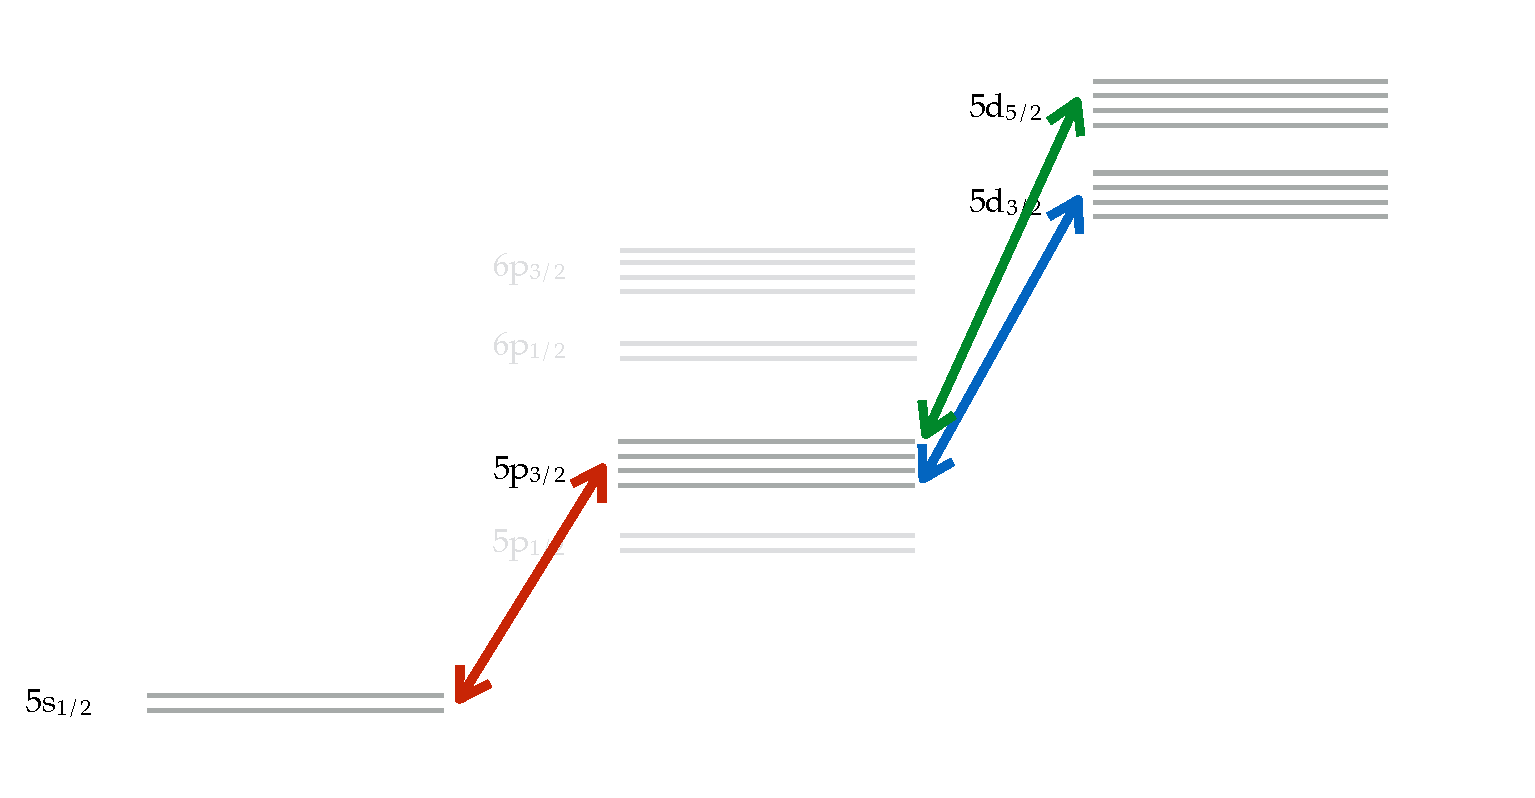
\includegraphics[width=\linewidth]
        {figs/05_twophoton/twophoton_level_scheme_coupling.pdf}
    \caption{
    Couplings of hyperfine manifolds included in the model. The laser is scanned
    across the $5^2\rm{S}_{\nicefrac{1}{2}} \rightarrow
    5^2\rm{P}_{\nicefrac{3}{2}}$ (\textsc{d2}) transition (red). The \textsc{d1}
    transition is too far from resonance and so is not coupled in the model. The
    same \textsc{d2} laser frequency couples $5^2\rm{P}_{\nicefrac{3}{2}}
    \rightarrow 5^2\rm{D_{\nicefrac{3}{2}}}$ and $5^2\rm{P}_{\nicefrac{3}{2}}
    \rightarrow 5^2\rm{D_{\nicefrac{3}{2}}}$ upper transitions.
    } 
    \label{fig:twophoton_level_scheme_coupling} 
    \end{figure}

    The manifolds involved in direct coupling are illustrated in figure
    \ref{fig:twophoton_level_scheme_coupling}. In the rotating frame
    description, eigenstates in the other manifolds are given zero energies, as
    they are not involved in the atom-light interaction part of the Hamiltonian.
    Note in particular that this includes the $5^2\rm{P}_{\nicefrac{1}{2}}$
    intermediate manifold. When we are near resonance with the \textsc{d2}
    transition, we assume that the \textsc{d1} resonance coupling frequency is
    far enough from resonance to be neglected.

    We see that this model is similar to a three-level system in the $\Xi$
    (ladder) configuration, but with a fourth level introducing an additional
    excited state manifold, forming a $\rm{Y}$ configuration. And of course in
    this case we have the added complexity of hyperfine structure included.

    The ladder is constrained in that it is the same field coupling the lower
    and upper transitions, so that the detunings only differ by constants. These
    are simply expressed as $\Delta_{12} = \Delta_{01} + \eta_{2}$ and
    $\Delta_{13} = \Delta_{01} + \eta_{3}$, where $\eta_{2} := (\omega_2 -
    \omega_1) - (\omega_1 - \omega_0) = \omega_2 - 2\omega_1$ and $\eta_{3} :=
    (\omega_3 - \omega_1) - (\omega_1 - \omega_0) = \omega_3 - 2\omega_1$.

  \subsection{Reducing the Transition Dipole Matrix Elements}

    Now that we have defined a Hilbert space basis and expressed the bare atomic
    Hamiltonian, the next step is to formulate the dipole operator. In order to
    do this we must compute the transition dipole matrix elements
    $\langle F m | d | F' m'_F \rangle$ coupling individual
    basis states.

    Calculating these matrix elements by integrating over the eigenstate
    wavefunctions explicitly is a computationally-intensive task. Fortunately,
    the spherical symmetry of the single-electron atom model allows us to use
    the spherical basis to factor out the angular part of the problem into
    coefficients that can be calculated much more quickly.

    The spherical vector basis for \textsc{3d} space is often more convenient
    than the Cartesian basis when dealing with angular momentum and spherical
    harmonics. The position vector $\mathbf{r}$ is given in this basis as
    \begin{equation}
      \mathbf{r} = r_- \hat{\mathbf{e}}_- + r_0 \hat{\mathbf{e}}_0 + 
        r_+ \hat{\mathbf{e}}_+
    \end{equation}
    where the basis unit vectors $\hat{\mathbf{e}}_-$, $\hat{\mathbf{e}}_0$ and
    $\hat{\mathbf{e}}_+$ are constructed as a complex linear combination of the
    Cartesian unit vectors
    \begin{align}
      \mathbf{e}_- &= \frac{\mathbf{e}_x - \rm{i} \mathbf{e}_y }{\sqrt{2}}, \\
      \mathbf{e}_0 &= \mathbf{e}_z, \\
      \mathbf{e}_+ &= \frac{-\mathbf{e}_x - \rm{i} \mathbf{e}_y }{\sqrt{2}}.
    \end{align}
    forming a complete orthonormal basis.

    The vector coordinates we then get from substitution, as
    \begin{align}
      r_- &= \frac{x + \rm{i} y }{\sqrt{2}} \\
      r_0 &= z \\
      r_+ &= \frac{-x + \rm{i} y }{\sqrt{2}}.
    \end{align}

    We label the components $r_-, r_0, r_+$ via the index $q \in \{ -1, 0, 1\}$.

    The Wigner-Eckart theorem\cite{wigner1959group,RevModPhys.2.305}, with the
    dipole operator a tensor of rank one, allows us to factor out the angular
    part of the dipole matrix elements such that they can be written in terms of
    Wigner symbols. Our derivation of the reduced dipole matrix elements will
    follow that given in Steck, 2007.\cite{Steck2007}

    Firstly the matrix elements can be factored such that the dependence on the
    $m_F$ and $m_F'$ quantum numbers is entirely within a Wigner 3-j factor, via
    the expression
    \begin{align}
      \langle F m_F | d_q | F' m'_F \rangle &= 
      \langle F  \| e \mathbf{r} \| F' \rangle \nonumber \\
      &\times (-1)^{F' - 1 + m_F} \sqrt{2F + 1}
      \begin{pmatrix}
        F' & 1 & F \\
        m_F' & q & -m_F 
      \end{pmatrix}
      \label{eqn:red_hf_tdme}
    \end{align}
    where $\langle F  \| e \mathbf{r} \| F' \rangle$ is now the reduced
    hyperfine dipole matrix element.

    We can go one step further in the reduction as the hyperfine transition
    couples states corresponding to different $\bf{F} = \bf{J} + \bf{I}$, but
    the dipole operator depends only on the position of the electron, not the
    nuclear state $\Ket{I m_I}$. We may thus factor out again
    \begin{align}
      \langle F  \| e \mathbf{r} \| F' \rangle =
      &\langle J  \| e \mathbf{r} \| J' \rangle \nonumber \\
      &\times (-1)^{F' + J + 1 + I}
      \sqrt{(2F' + 1)(2J + 1)}
            \begin{Bmatrix}
        J & J' & 1 \\
        F' & F & I 
      \end{Bmatrix}
      \label{eqn:red_tdme}
    \end{align}
    where now the dependence on $F$ and $F'$ is also factored out of the reduced
    fine structure matrix element $\langle J  \| e \mathbf{r} \| J' \rangle$ and
    the angular dependence of the dipole matrix element is given by the Wigner
    6-j coefficient, which can be calculated easily.

    \begin{table}
      \centering
      \begin{tabular}{ l r r r }
        \hline
        $n L_J$ & $n' L'_{J'}$ & $\Gamma_{J, J'}$ & 
        $\langle J  \| e \mathbf{r} \| J' \rangle$  \\
        \hline      
        $5\rm{S}_{\nicefrac{1}{2}}$ & $5\rm{P}_{\nicefrac{1}{2}}$ 
          & 5.750 & 3.007 \\
        $5\rm{S}_{\nicefrac{1}{2}}$ & $5\rm{P}_{\nicefrac{3}{2}}$ 
          & 6.067 & 4.245 \\
        % $5\rm{S}_{\nicefrac{1}{2}}$ & $6\rm{P}_{\nicefrac{1}{2}}$ 
        %   &  & ** \\
        % $5\rm{S}_{\nicefrac{1}{2}}$ & $6\rm{P}_{\nicefrac{3}{2}}$ 
        %   &  & ** \\
        \noalign{\medskip}
        $5\rm{P}_{\nicefrac{1}{2}}$ & $5\rm{D}_{\nicefrac{3}{2}}$ 
          & 0.4756 & 1.143 \\
        \noalign{\medskip}
        $5\rm{P}_{\nicefrac{3}{2}}$ & $5\rm{D}_{\nicefrac{3}{2}}$ 
          & 0.1068 & 0.3935 \\
        $5\rm{P}_{\nicefrac{3}{2}}$ & $5\rm{D}_{\nicefrac{5}{2}}$ 
          & 0.6266 & 1.167 \\
        \noalign{\medskip}
        $6\rm{P}_{\nicefrac{1}{2}}$ & $5\rm{D}_{\nicefrac{3}{2}}$ 
          & 0.209 & 12.87 \\
        \noalign{\medskip}
        $6\rm{P}_{\nicefrac{3}{2}}$ & $5\rm{D}_{\nicefrac{3}{2}}$ 
          & 0.03770 & 4.103 \\
        $6\rm{P}_{\nicefrac{3}{2}}$ & $5\rm{D}_{\nicefrac{5}{2}}$ 
          & 0.2273 & 12.31 \\
        \hline  
      \end{tabular}
      \caption{
      Spontaneous Decay Lifetimes (ns) and reduced transition dipole matrix
      elements ($e a_0$) for fine structure transitions relevant to the model.
      Decay lifetimes are from Safronova, 2011 and Sansonetti,
      2006\cite{Sansonetti2006,Safronova2011} and transition dipole matrix
      elements are calculated from the lifetimes via equation
      (\ref{eqn:tdme_from_width}).
      }
      \label{tab:exp_widths}
    \end{table}

    The reduced fine structure matrix element must be calculated theoretically
    by integrating over the radial parts of the atomic wavefunction in a
    suitable basis for the required accuracy. Alternatively, and better for our
    purposes, it can be determined experimentally via the
    relation\cite{loudon2000quantum}
    \begin{equation}
      \Gamma_{J, J'} = \frac{\omega_0^3}{3 \pi \varepsilon_0 \hbar c^3} 
        \frac{2J + 1}{2 J' + 1} \left| \langle J  \| e \mathbf{r} \| J' 
        \rangle \right|^2
      \label{eqn:tdme_from_width}
    \end{equation}

    where $\Gamma_{J, J'}$ is the spontaneous decay rate from the fine structure
    manifold $J'$ to a lower state $J$. The factor $(2J + 1)/(2 J' + 1)$
    accounts for the degeneracy of the fine structure manifolds. These decay
    rates may be measured and thus used to derive transition dipole
    matrix elements. Lifetimes and dipole matrix elements for the transitions
    relevant to our model are listed and referenced in table
    \ref{tab:exp_widths}.

  \subsection{Selection Rules}

    An additional benefit of the Wigner-Eckart theory is that the coefficients
    vanish unless certain conditions are met, meaning that forbidden transitions
    can be identified without time-consuming calculation.

    In particular, the 3-j symbol in equation (\ref{eqn:red_hf_tdme}) is zero
    if the magnetic quantum numbers do not satisfy the relation $m_F = m_F' +
    q$ for $q \in \{ -1, 0, 1\}$. The full hyperfine selection rules are
    \begin{align}
      F' = F &\textrm{~or~} F' = F \pm 1 \nonumber \\
      m_F' = m_F &\textrm{~or~} m_F' = m_F \pm 1 \\
      F' \ne F &\textrm{~if~} m_F' = m_F. \nonumber     
    \end{align}    

  \subsection{The Interaction Hamiltonian}

    Now that we have expressed the transition dipole matrix elements, we can put
    together the dipole operator and form the interaction Hamiltonian.

    To begin with we will consider a single fine structure transition, coupling
    a lower energy manifold $nJ$ to a higher energy manifold $n'J'$. This could
    for example represent coupling just on the \textsc{d2} transition from
    $5^2\rm{S}_{\nicefrac{1}{2}}$ to $5^2\rm{P}_{\nicefrac{3}{2}}$.
    We will be able to extend the analysis to further levels later.

    The projection operators for the sublevels in a given manifold can now be
    summed over the hyperfine quantum numbers and the magnetic sublevel indices,
    and expressed as
    \begin{align}
      P = \sum_{F m_F} \Ket{F m_F} \Bra{F m_F} \nonumber \\
      P' = \sum_{F' m'_F} \Ket{F' m'_F} \Bra{F' m'_F}.
      \label{eqn:hf_projection}
    \end{align}

    Our restricted Hilbert space then consists of the two coupled manifolds. The
    identity is $P + P'$ and the dipole operator is then given by
    \begin{align}
      d_q &= (P + P') d_q (P + P') \\
          &= P d_q P' + P d_q P' \\
          &= d_q^{(+)} + d_q^{(-)}.
    \end{align}
    We then expand these terms with (\ref{eqn:hf_projection}) to find
    \begin{align}
      d^{(+)}_q &= P d_q P' \nonumber \\
      &= \sum_{F m_F F' m'_F} \langle F m | d_q | F' m'_F 
        \rangle \Ket{F m_F} \Bra{F' m'_F}
    \end{align}
    and then introduce the reduced dipole matrix element from (\ref{eqn:red_tdme})
    to obtain
    \begin{align}
      d^{(+)}_q &= \sum_{F m_F F' m'_F} \langle J  \| e \mathbf{r} \| J' \rangle 
      (-1)^{F' + J + 1 + I} \sqrt{(2F + 1)(2J + 1)} 
      \begin{Bmatrix}
        J & J' & 1 \\
        F' & F & I 
      \end{Bmatrix} \nonumber \\
      & \times \langle F m_F | F' m'; 1 q \rangle \Ket{F m_F} \Bra{F' m'_F}.
    \end{align}
    Applying the same for $d_q^{(-)}$ one can show that
    \begin{equation}
      d^{(-)}_q = (-1)^q (d_q^{(+)})^\dag.
    \end{equation}

    It is useful to define a weighted lowering operator to account for the
    angular dependence factors
    \begin{align}
      \Sigma_q &= \sum_{F m_F F' m'_F} (-1)^{F' + J + 1 + I}
        \sqrt{(2F + 1)(2J + 1)} 
        \begin{Bmatrix}
          J & J' & 1 \\
          F' & F & I 
        \end{Bmatrix} \nonumber \\
        & \times \langle F m_F | F' m'; 1 q \rangle \Ket{F m_F} \Bra{F' m'_F}
    \end{align}
    which then allows us to write the dipole operator as 
    \begin{align}
      d_q &= d_q^{(+)} + d_q^{(-)} \nonumber \\
          &= \langle J  \| e \mathbf{r} \| J' \rangle \left[ \Sigma_q + 
            (-1)^q \Sigma_{-q}^\dag \right]
    \end{align}
    The interaction Hamiltonian, in the same way we derived in chapter \ref{chp:propagation} for the two-level description, becomes
    \begin{equation}
      \mathcal{H}_\Omega = - \left( \mathbf{d}^{(+)} \cdot \mathcal{E}^{(-)} + 
        \mathbf{d}^{(-)} \cdot \mathcal{E}^{(+)} \right).
    \end{equation}


    We define the fine structure manifold Rabi frequency as 
    \begin{equation}
      \Omega_q := \frac{\langle J  \| e \mathbf{r} \| J' \rangle E^+_q(0)}{\hbar}
    \end{equation}
    such that the interaction Hamiltonian can be written in the simple form
    \begin{equation}
      \mathcal{H}_\Omega = \frac{\hbar}{2} \sum_q \left[ \Omega^*_q \Sigma_q + 
        \Omega_q \Sigma_q^\dag \right]
    \end{equation}

    Now for the two-photon Y-configuration, we have more than one transition to
    consider, as was illustrated in figure
    \ref{fig:twophoton_level_scheme_coupling}. Using the same indexing as
    before,  with levels $\{ 5^2\rm{S}_{\nicefrac{1}{2}},
    5^2\rm{P}_{\nicefrac{3}{2}}, 5^2\rm{D}_{\nicefrac{3}{2}},
    5^2\rm{D}_{\nicefrac{5}{2}} \}$ represented by $i = {0,1,2,3}$
    respectively, we can write the total interaction part of the Hamiltonian as
    \begin{equation}
      \mathcal{H}_{\Omega} = \frac{\hbar}{2} \sum_q \left[ \Omega^*_{01,q} 
      \Sigma_{01,q} + \Omega^*_{12,q} \Sigma_{12,q} + \Omega^*_{13,q} 
      \Sigma_{13,q} + \hc \right] 
    \end{equation}

    The total Hamiltonian is then given by
    \begin{equation}
      \mathcal{H} = \mathcal{H}_0' + \mathcal{H}_\Omega.
    \end{equation}

  \subsection{Spontaneous Decay and the Master Equation} % (fold)    

    At this point we have have defined all the necessary parameters required to
    follow coherent evolution of the atomic system during the atom light
    interaction. We recall that the set of equations we hope to solve are those
    defined by the Lindblad master equation, derived in appendix
    \ref{apx:qu_dyn},
    \begin{equation}\label{eqn:lindblad_twophoton}
      \ii \hbar \frac{\partial \rho}{\partial t} = [\mathcal{H}, \rho] + 
        \mathcal{L}\left\{ \rho \right\}
    \end{equation}
    where the Lindblad term accounting for dissipation is given by
        \begin{equation}
      \mathcal{L}\left\{ \rho \right\} = 
        \sum_j{C_j \rho C_j^\dagger - \tfrac{1}{2}\left(\rho C_j^\dagger C_j + 
            C_j^\dagger C_j \rho \right)}.
      \label{eqn:lindblad_op_twophoton}
    \end{equation}   

    Our remaining task is to define the set of collapse operators $C_j$ for the
    system defining spontaneous decay of excited states to lower states,
    including the included angular momentum structure. We are able to use the
    same lowering operator $\Sigma_q$ to account for the branching factors to
    each hyperfine sublevel, and the collapse operators are then given by
    \begin{equation}
      C_{J' \rightarrow J} = \sqrt{\Gamma_{J,J'}} 
        \left( \frac{2J' + 1}{2J + 1} \right)  \sum_q \Sigma_q
    \end{equation}
    for each decay channel $J' \rightarrow J$ allowed by fine structure
    selection rules.

    \begin{figure}[]
    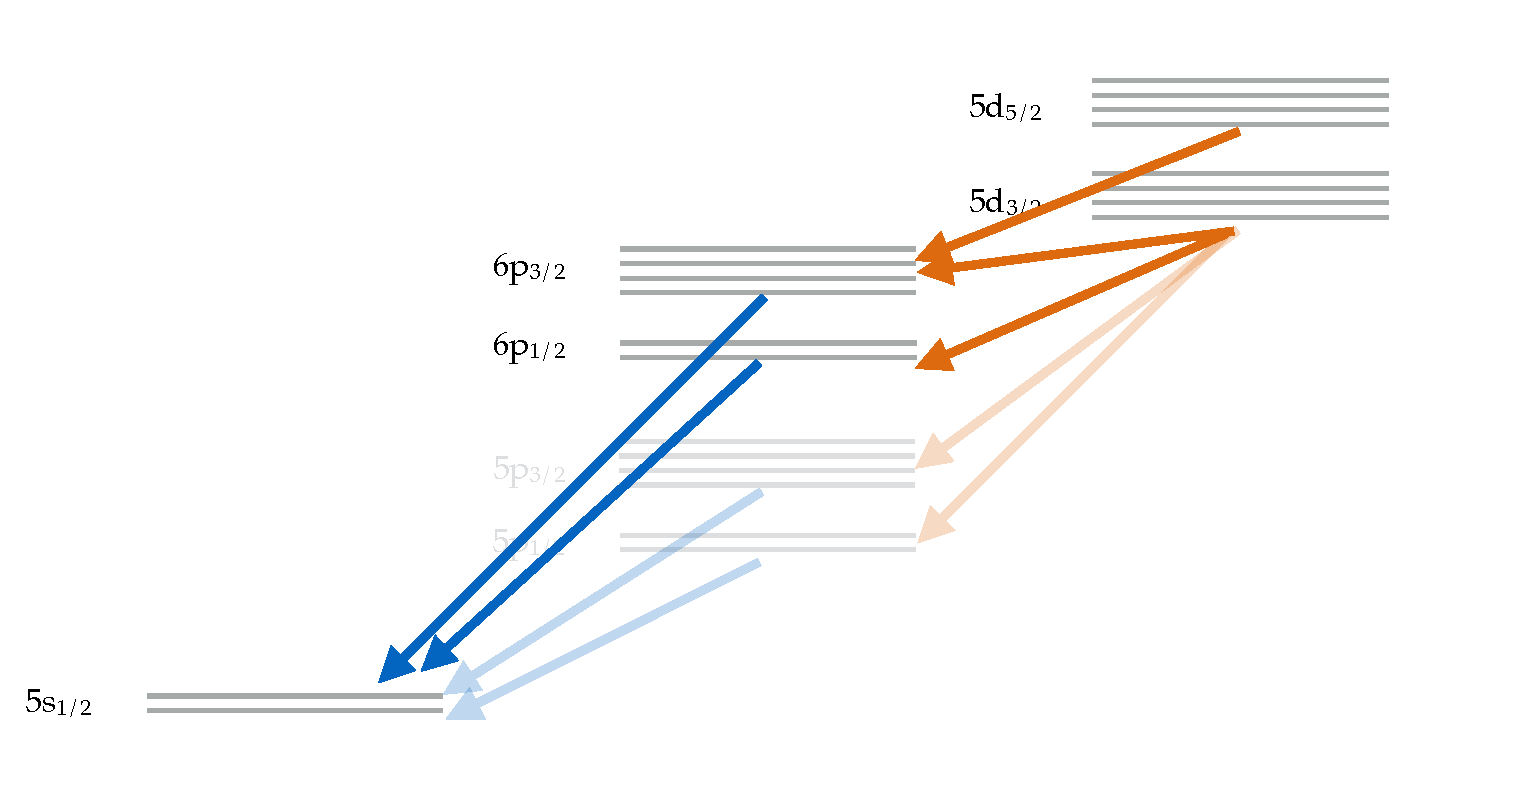
\includegraphics[width=\linewidth]
        {figs/05_twophoton/twophoton_level_scheme_decay_2.pdf}
    \caption{
    Decay channels of selected hyperfine manifolds in rubidium.  Blue
    flourescence is from the decay from $6^2\rm{P}_{\nicefrac{1}{2}}$ and
    $6^2\rm{P}_{\nicefrac{3}{2}}$ to the $5\rm{S}$ ground state. The $6\rm{P}$
    states in this model are populated via decay from the
    $5^2\rm{D}_{\nicefrac{3}{2}}$ and $5^2\rm{D}_{\nicefrac{5}{2}}$ states.
    Branching from $5^2\rm{D}_{\nicefrac{3}{2}}$ down to the $5\rm{P}$ states
    and from the $5\rm{P}$ states to the $5\rm{S}$ ground state are also
    included in the model.
    } 
    \label{fig:twophoton_level_scheme_decay} 
    \end{figure}

    The allowed decay channels for the manifolds included in our model are
    illustrated in figure \ref{fig:twophoton_level_scheme_decay}. It is
    important to note that the $6\rm{P}$ states in fact have decay channels to
    states other than the ground state $5^2\rm{S}_{\nicefrac{1}{2}}$ which are
    not included in this model. We here assume that all of the $6\rm{P}$
    population decays via a single channel to the ground state. The decay widths
    $\Gamma_{J,J'}$ are given in table \ref{tab:exp_widths}.
